\chapter[Metodologia]{Metodologia}

O interesse desse capítulo é responder como os objetivos desse trabalho serão
alcançados e como a solução do problema de pesquisa será abordado. As seguintes
seções são apresentadas: seção \ref{sec:classificacao}, apresenta o tipo de
metodologia de pesquisa utilizada no desenvolvimento desse trabalho; seção \ref{sec:modelagem}, especifíca o planejamento, atividades, e fluxo de execução;
seção \ref{sec:cronograma}, apresenta o cronograma; seção \ref{sec:provaconceito},
detalha a prova de conceito.

\section{Classificação da Pesquisa}
\label{sec:classificacao}

Para a classificação de um tipo de pesquisa, é necessário a definição clara de critérios baseados nos objetivos e procedimentos a serem seguidos \cite{gil2002}. Os tipos de pesquisa baseadas nos objetivos são usualmente classificadas em três grupos: exploratória, descritiva e explicativa \cite{gil2002}.

A pesquisa exploratória é definida por Theodorson e Theodorson como sendo um estudo preliminar com o objetivo principal de se familiarizar com o tópico abordado, de modo que o estudo posterior possa ser realizado com maior compreensão e precisão. Theodorson e Theodorson também esclarecem que a pesquisa exploratória permite que o pesquisador defina o seu problema de pesquisa e formule hipóteses mais precisas, tornando possível a escolha de técnicas mais adequadas e gerando alertas para quais as potenciais dificuldades e sensibilidades da área \cite{theodorson1970}.

De acordo com Fonseca, a pesquisa descritiva é utilizada quando o pesquisador tem conhecimento prévio do assunto e possui interesse em descrever um fenômeno. A partir desse conhecimento prévio, o pesquisador pode formular hipóteses, podendo confirmá-las ou não \cite{fonseca2002}.

Já a pesquisa explicativa tem como objetivo central identificar fatores que determinam ou contribuem para a ocorrência de fenômenos. Esse tipo de pesquisa explica o porquê a razão, o motivo de acontecimentos \cite{gil2002}.

Dado os objetivos de estudo e contexto desse trabalho, a metodologia de pesquisa escolhida foi a pesquisa exploratória.

\section{Modelagem do Fluxo de Atividades}
\label{sec:modelagem}

O Diagrama a seguir \ref{figura:diagram}, desenvolvido utilizando o BPMN2
\textit{Modeler Plugin} para Eclipse \cite{eclipse}, ilustra a condução das atividades
requeridas para o desenvolvimento do TCC 1, e as planejadas para o TCC 2. As
descrições das atividades presentes no diagrama são apresentadas em seguida.


\begin{figure}[H]
  \centering
  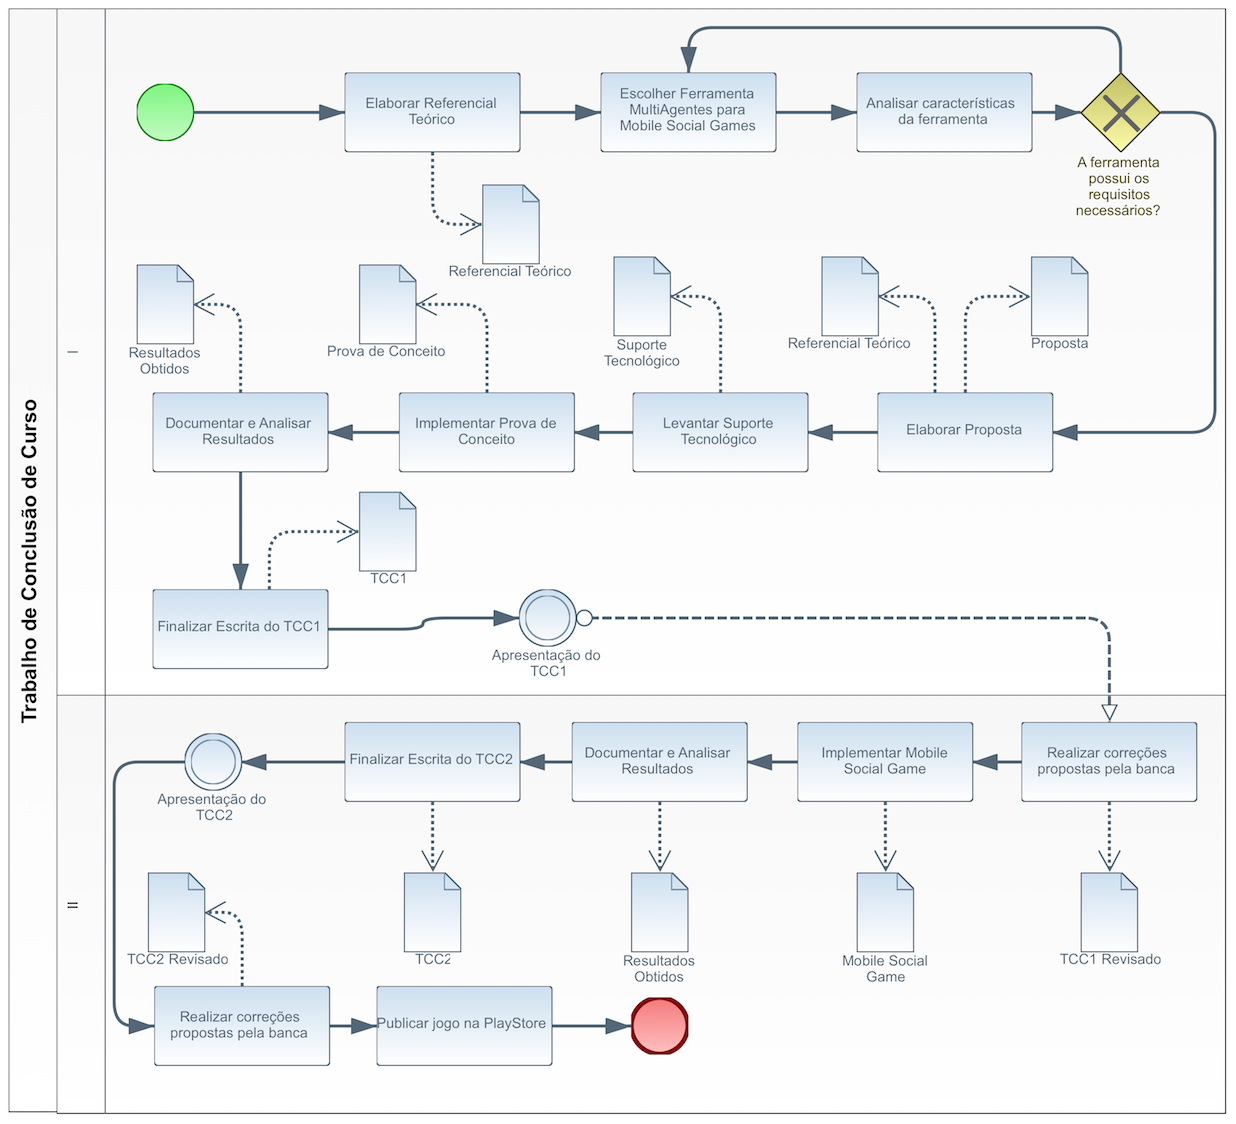
\includegraphics[width=16cm]{figuras/diagram2}
  \caption{Fluxo de atividades do TCC}
  \label{figura:diagram}
\end{figure}

Atividades mapeadas para o TCC 1:

\textbf{Elaborar referencial teórico:} teve como objetivo construir o conhecimento
base para a elaboração do trabalho. Através do mapeamento da literatura, publicações,
e autores.

\textbf{Escolher ferramenta MultiAgentes para \textit{Mobile Social Games}:} teve
como objetivo a pesquisa, e escolha de uma ferramenta que aplicasse o paradigma
MultiAgentes no contexto de \textit{Mobile Social Games}. Essa pesquisa obteve como
resultado uma única ferramenta, o AMUSE, descrito detalhadamente no capítulo de Suporte Tecnológico.

\textbf{Analisar características da ferramenta:} teve como objetivo analisar as
características e restrições da ferramenta escolhida, no caso, o AMUSE.

\textbf{Elaborar proposta:} teve como objetivo a definição de uma proposta que
contemplasse os objetivos deste trabalho de conclusão de curso. Essa proposta foi
composta de uma visão geral dos objetivos, e uma visão técnica arquitetural.

\textbf{Levantar suporte tecnológico:} teve como objetivo o levantamento das
das ferramentas de suporte necessárias para a elaboração desse trabalho.

\textbf{Implementar prova de conceito:} teve como objetivo a implementação da
prova de conceito para provar a viabilidade técnica desse trabalho. E que poderá
ser utilizada em parte no desenvolvimento da proposta.

\textbf{Documentar e analisar resultados:} teve como objetivo a formalização dos
resultados obtidos no desenvolvimento da prova de conceito.

\textbf{Finalizar escrita do TCC 1:} teve como objetivo o refinamento do trabalho,
e adição de observações pertinentes para entrega a banca avaliadora.

Atividades mapeadas para o TCC 2:

\textbf{Realizar correções propostas pela banca:} possui como objetivo a correção
dos pontos levantados pela banca avaliadora.

\textbf{Implementar \textit{Mobile Social Game}:} possui como objetivo a
implementação da proposta feita no TCC 1.

\textbf{Documentar e analisar resultados:} possui como objetivo a documentação e
análise dos resultados obtidos com o desenvolvimento da proposta, e evolução do
projeto.

\textbf{Finalizar escrita do TCC 2:} possui como objetivo o refinamento do trabalho,
e adição de observações pertinentes para entrega a banca avaliadora.

\textbf{Publicar jogo na Google Play:} possui como objetivo a monetização da proposta
desenvolvida através da publicação na plataforma Google Play.


\section{Cronograma de Pesquisa}
\label{sec:cronograma}

O cronograma seguido para o desenvolvimento desse trabalho pode ser observado na Tabela 1 e Tabela 2. A Tabela 2, referente ao cronograma do TCC 2, é passível de mudanças de acordo com o andamento do trabalho.

%Cronograma 1
\begin{table}[H]
\centering
\resizebox{\textwidth}{!}{%
\begin{tabular}{|l|l|c|c|c|l|c|}
\hline
\multicolumn{1}{|c|}{\textbf{Atividade}} & \multicolumn{1}{c|}{\textbf{Janeiro}} & \textbf{Fevereiro} & \textbf{Março} & \textbf{Abril} & \textbf{Maio} & \textbf{Junho} \\ \hline
Levantamento Bibliográfico & \multicolumn{1}{c|}{X} & X & X & \multicolumn{1}{l|}{} &  &  \\ \hline
Definição do Escopo &  & X & X & \multicolumn{1}{l|}{} &  &  \\ \hline
Levantamento do Suporte Tecnológico &  & X & X & \multicolumn{1}{l|}{} &  &  \\ \hline
Implementar Prova de Conceito &  &  & X & X & \multicolumn{1}{c|}{X} &  \\ \hline
Análise de Resultados &  & \multicolumn{1}{l|}{} & X & \multicolumn{1}{c|}{X} & \multicolumn{1}{c|}{X} &  \\ \hline
Escrita do TCC 1 &  & \multicolumn{1}{l|}{} & X & X & \multicolumn{1}{c|}{X} & X \\ \hline
Apresentação do TCC 1 &  & \multicolumn{1}{l|}{} & \multicolumn{1}{l|}{} &  &  & \multicolumn{1}{c|}{X} \\ \hline
Realizar correções requisitadas pela banca &  & \multicolumn{1}{l|}{} & \multicolumn{1}{l|}{} & \multicolumn{1}{l|}{} &  & \multicolumn{1}{c|}{X} \\ \hline
\end{tabular}
}
\caption{Cronograma TCC 1}
\label{my-label}
\end{table}


% Cronograma 2
\begin{table}[H]
\centering
\resizebox{\textwidth}{!}{%
\begin{tabular}{|l|l|l|c|c|}
\hline
\multicolumn{1}{|c|}{\textbf{Atividade}}   & \multicolumn{1}{c|}{\textbf{Junho}} & \multicolumn{1}{c|}{\textbf{Julho}} & \textbf{Agosto}       & \textbf{Setembro} \\ \hline
Implementar Mobile Social Game             & \multicolumn{1}{c|}{X}              & \multicolumn{1}{c|}{X}              & X                     &                   \\ \hline
Documentar e Analisar Resultados           &                                     &                                     & X                     & X                 \\ \hline
Escrita do TCC 2                           &                                     &                                     & X                     & X                 \\ \hline
Apresentação do TCC 2                      &                                     &                                     & \multicolumn{1}{l|}{} & X                 \\ \hline
Realizar correções requisitadas pela banca &                                     &                                     & \multicolumn{1}{l|}{} & X                 \\ \hline
\end{tabular}
}
\caption{Cronograma TCC 2}
\label{my-label}
\end{table}

\section{Prova de Conceito}
\label{sec:provaconceito}

Dado o contexto de estudo desse projeto, é necessário a integração de várias
plataformas que utilizam tecnologias distintas. A avaliação dos possíveis
riscos de integração dessas plataformas é pertinente no atual momento do
projeto, pois ocorre em um estágio inicial de desenvolvimento.

Para provar a viabilidade técnica do desenvolvimento da proposta, foi elaborada
uma prova de conceito, que possui como objetivo principal a integração das
várias plataformas presentes na proposta desse projeto. As subseções
\ref{subsec:descconceito}, \ref{subsec:configambiente} e
\ref{subsec:integracaoplataformas} detalham a Descrição da Prova de Conceito,
Configuração do Ambiente de Desenvolvimento, e Integração Entre Plataformas,
respectivamente.

  \subsection{Descrição da Prova de Conceito}
  \label{subsec:descconceito}
  A pesquisa exploratória realizada, juntamente com o referencial teórico
  levantado, revelou que será necessário a utilização das plataformas: JADE,
  WADE, AMUSE e Android para a aplicação do paradigma MultiAgentes em
  \textit{Mobile Social Games}.

  Para validar as integrações entre as plataformas mencionadas anteriormente,
  proporcionar a configuração do ambiente de desenvolvimento, e criar um
  subsídio reutilizável para o desenvolvimento da proposta, capítulo
  \ref{chapter:proposta}, a seguinte Prova de Conceito foi planejada: uma
  versão inicial de controle de \textit{login} de usuários através de nome e
  senha.

  Esta primeira versão de controle de \textit{login} poderá ser reutilizada na
  proposta, permitirá que os fluxos de integração entre as plataformas seja
  validado, e o ambiente de desenvolvimento seja configurado.

  O tópico a seguir descreve os passos necessários para a configuração do
  ambiente de desenvolvimento, utilizando como base as ferramentas de
  desenvolvimento, seção \ref{sec:tecferramentasdesenvolvimento}.

  TODO
  % Descrição arquitetural
  % JADE - WADE - AMUSE - BANCO - APP

  \subsection{Configuração do Ambiente de Desenvolvimento}
  \label{subsec:configambiente}

  Para realizar o desenvolvimento da Prova de Conceito, utilizou-se de uma
  máquina com as seguintes especificações: processador 2.6 GHz Intel Core i5,
  memória ram de 16 GB 1600 MHz DDR3 e sistema operacional MacOS Sierra 10.12.5.

  O primeiro passo para a configuração do ambiente foi a verificação da
  existência do Java \cite{java}, e Apache Ant \cite{ant} na máquina de
  desenvolvimento. Visto que as plataformas utilizadas nesse projeto
  necessitam dessas duas tecnologias para a configuração base.

  Após a verificação da existência do Java, seguiu-se os passos disponíveis para
  a configuração do AMUSE. Tais passos estão disponíveis no tutorial de
  configuração, disponível em:
  \url{http://jade.tilab.com/amuse/doc/Amuse-Startup-Guide.doc}.

  % Mostrar banco inicializado
  % Mostrar setup do wade e amuse

  TODO

  \subsection{Integração Entre Plataformas}
  \label{subsec:integracaoplataformas}
  TODO

\section{Considerações Finais do Capítulo}

O objetivo desse capítulo foi apresentar a metodologia utilizada no desenvolvimento
desse trabalho de conclusão de curso. Esse capítulo possui a classificação do tipo
de pesquisa, modelagem do fluxo de atividades, cronograma, e prova de conceito para
evolução da proposta desse TCC.
